\documentclass[a4paper,11pt]{report}
\usepackage[T1]{fontenc}
\usepackage[utf8]{inputenc}
\usepackage{lmodern}
\usepackage[francais]{babel}
\usepackage{graphicx}
\usepackage{setspace}
\usepackage{float}
\usepackage{pdfpages} 

\title{Recette du projet : MonsterShip}
\author{Olivier \bsc{Boissard}, Kevin \bsc{Boulala},\\Maxime \bsc{Dubois}, Antoine \bsc{Lavier}}

\begin{document}

\maketitle
\setcounter{tocdepth}{1}
\tableofcontents

\chapter{Introduction}
  Dans ce rapport, nous allons faire la recette du projet MonsterShip commencé le 16 Décembre 2015. Nous verrons ce qui était prévu, ce qui a été implémenté et comment les fonctionnalités ont été implémenté. Suivi des fonctionnalités manquantes, les idées qui sont venues au cours du développement, et un bilan de ce que nous avons appris avec cette expérience.
  
\chapter{Contexte}
  Dans le cadre de nos études de Master 2 Informatique, nous avons eu pour mission dans le module de Programmation d'Applications Distribuées de travailler en groupe à l'élaboration d'un projet utilisant JavaEE avec le serveur d'application WildFly puis de le développer. L'objectif est de développer un jeu accessible depuis un navigateur. Le cahier des charges que nous avons écrit pour l'occasion est disponible en annexe.

\chapter{Description de MonsterShip}
  MonsterShip est un space opera se déroulant dans la zone de Sagittarius A*, au centre de notre galaxie. Nous contrôlons un vaisseau dont l'équipage est composé de monstres. Pour améliorer le vaisseau, nous utilisons comme ressource première l'équipage qui fusionne avec la structure du vaisseau. Mais il faut aussi un certain nombre de monstres par module pour qu'il fonctionne correctement. Pour renouveler son équipage et donc d'augmenter la puissance de son vaisseau, il faut aller récolter des monstres sur des planètes ou des vaisseaux laissés à l'abandon par d'autres joueurs.

\chapter{Le développement}

  \section{La structure du projet}

    \subsection{Organisation du projet}
      Voici l'arobrescence du projet MonsterShip :
      \begin{description}
        \item[MonsterShip] racine du projet
        \begin{description}
          \item[monstership-ear] archive pour déployer l'application
          \item[monstership-ejb] src/main/java/com/monstership/
          \begin{description}
            \item[data] définit l'accès aux données
            \item[model] définit la structure de données du projet
            \item[service] gère les fonctionnalités de l'application 
            \item[util] outillage
          \end{description}
          \item[monstership-web] l'application web
          \begin{itemize}
            \item src/main/java/com/monstership/
            \begin{description}
              \item[controller]
              \item[rest]
              \item[util] 
            \end{description}
            \item src/main/webapp/
            \begin{description}
              \item[resources] 
              \item[WEB-INF]
              \item[./] 
            \end{description}
          \end{itemize}
          
          
        \end{description}
      \end{description}

    \subsection{Les technologies utilisées}

  \section{Les fonctionnalités implémentées}

    \subsection{Connexion et inscription}
  
      \paragraph{Description}
        Pour commencer un visiteur peut accéder depuis la page d'accueil de MonsterShip (qui est la page de connexion) à la page d'inscription. Il n'y a que deux champs : un premier pour le login, un second pour le mot de passe. Le login doit être unique et le mot de passe doit contenir entre 8 et 25 caractères.
        \begin{figure}[H]
          \begin{center}
            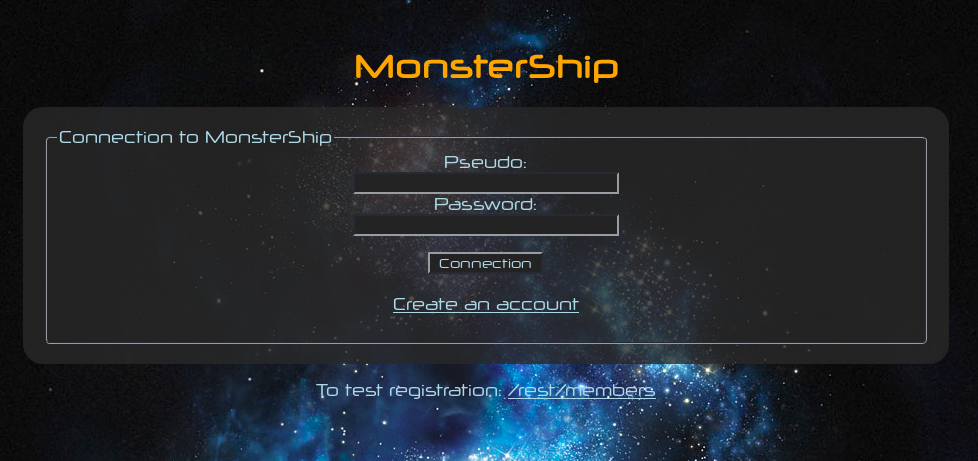
\includegraphics[width=.8\textwidth]{images/connexion.png}
            \caption{Écran de connexion}
            \label{fig:ec_co}
          \end{center}
        \end{figure}
        \begin{figure}[H]
          \begin{center}
            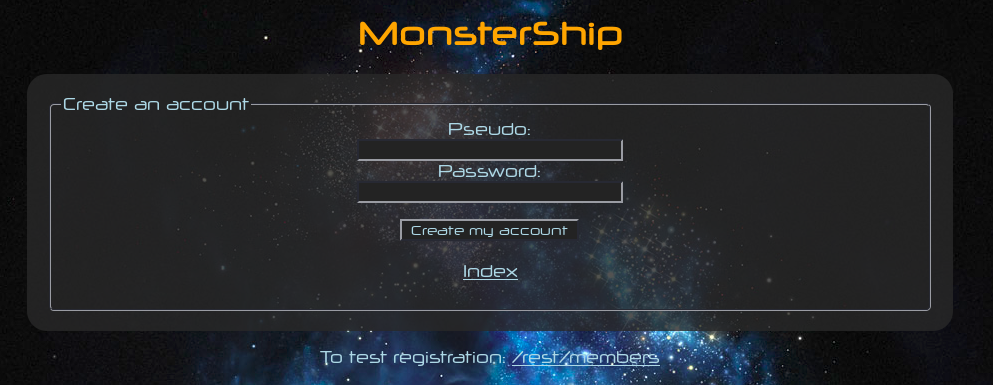
\includegraphics[width=.8\textwidth]{images/inscription.png}
            \caption{Écran d'inscription}
            \label{fig:ec_inc}
          \end{center}
        \end{figure}
        
      \paragraph{Implémentation}
        Nous avons créé une interface local à l'EJB pour gérer les connexions et les inscriptions : \textit{"IMemberManagerLocal"}. Cette interface propose les prototypes de deux méthodes : une première pour la connexion \textit{"Member connect(Member member) throws Exception"} et une seconde pour l'inscription \textit{"Member register(Member member) throws Exception"}.\\
        Cette interface a été implémenté dans \textit{"MemberManager"}. Pour ces deux méthodes nous récupérons en paramètre un Member dont on verra d'où il vient plus tard dans cette partie. Pour la connexion nous utilisons l'EntityManager pour créer une requête qui récupèrera l'utilisateur dans la base de donnée. Cette requête cherche un utilisateur selon le pseudonyme et le mot de passe que nous avons dans l'objet de type Member (reçu en paramètre d'entrée). Puis nous retournons le Member que la requête a permis de trouver, si aucun Member n'est trouvé, nous lançons une exception.\\
        Pour l'inscription nous utilisons l'\textit{"EntityManager"} pour inscrire le Member (le rendre persistant) dans la base de donnée.\\
        
        Du côté de l'application web, nous avons une page qui contient un formulaire avec un commandButton ayant pour action de faire un appel à un \textit{"MemberController"} et notamment de sa méthode connect. C'est de cette manière qu'on récupère un Member : l'inputText du formulaire récupère la valeur avec \textit{"newMember.pseudo"} (et de même avec le mot de passe).\\
        
        Il faut ensuite faire le lien entre les Manager que nous venons de développer et l'application web. Pour cela on crée des Controller : notamment ici un \textit{"MemberController"} qui a comme attribut l'EJB IMemberManagerLocal. Le newMember que nous avions dans le formulaire est récupéré par ce controller, puis est passé à l'EJB et à son MemberManager. La méthode de connexion du Manager retournant un Member ou lançant une exception, nous redirigeons l'utilisateur sur la page principale du jeu s'il peut se connecter, sinon nous capturons l'exception et nous retournons un message à la page web grâce aux FacesContext. Et nous faisons de même avec l'inscription.
      

    \subsection{Visualisation de la carte et déplacements}


\chapter{La suite}

  \section{Les fonctionnalités attendues}
      Une fois l'utilisateur connecté (après une connexion ou une inscription valide), l'utilisateur accède à certaines informations de son vaisseau et à la map de la zone où il se trouve.
      Nous affichons le nom du commander, les coordonnées de son vaisseau, son équipage et le nombre de points d'action qu'il lui reste. Ces informations sont mises à jour dynamiquement à chaque déplacement.
      Pour se déplacer, l'utilisateur doit cliquer sur les cases de la carte en sachant qu'il ne peut se déplacer qu'horizontalement ou verticalement. De même l'affichage de la carte est dynamique.
      \begin{figure}[H]
        \begin{center}
          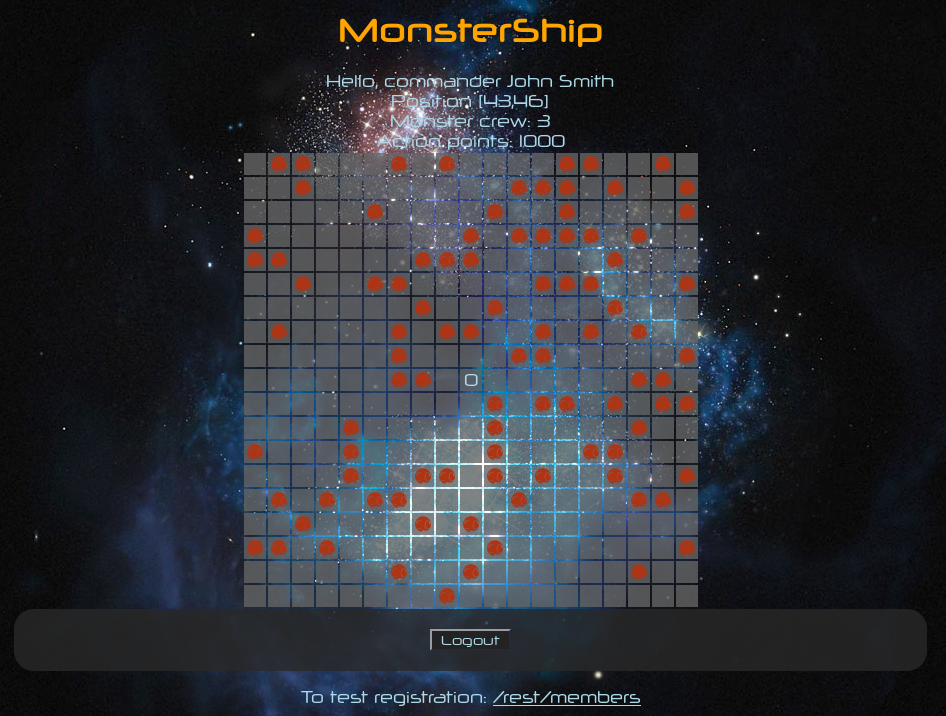
\includegraphics[width=.8\textwidth]{images/home.png}
          \caption{Écran principal du jeu}
          \label{fig:ec_home}
        \end{center}
      \end{figure}

    

\chapter{La suite}

  \section{Les fonctionnalités non implémentées}
    Certaines fonctionnalités prévues ne sont pas encore implémentées. 
    Par exemple, nous n'avons pas eu le temps d'implémenter l'amélioration du vaisseau ni les combats entre les joueurs.
    De même un joueur ayant perdu trop de combat et qui se retrouve avec un vaisseau trop endommagé doit pouvoir l'abandonner.
    
    \subsection{Récolte de monstres}
      Pour améliorer le vaisseau, il faut le fusionner avec un certain nombre de membres d'équipages. Ceci implique que le joueur doit pouvoir en récupérer.
      Pour cela, le plus simple est d'en recruter sur des planètes habitées. Le joueur doit donc se rendre sur une de ses planètes.
      Après être allé au bon endroit, il dispose de deux solutions.
      La première consiste à utiliser des points d'actions. Le joueur peut choisir le nombre de points d'actions qu'il souhaite utiliser.
      Plus il investira de points d'actions, plus il récupèrera de monstres.
      \newline
      La seconde solution pour récupérer des monstres consiste à rester longtemps à la surface de la planète. Dans ce cas, le joueur n'utilise pas de points d'actions, et plus les garder pour se déplacer ou attaquer d'autres joueurs.
      Le nombre de monstres récupéré dépendra uniquement du temps à la surface de la planète, ce qui peut donc être bien plus rentable.
      Toutefois cette solution n'est pas sans risques. En effet, le joueur choisit au départ combien de temps il doit rester pour récupérer des monstres.
      Comme il ne pourra pas partir avant la fin du timer, il s'expose aux attaques sans pouvoir se défendre ou s'enfuir. Il risque donc de perdre plus de monstres qu'il n'en récupèrera.
      De plus, il peut également se retrouver avec un vaisseau gravement endommagé.
    
    \subsection{Améliorations du vaisseau}
      Ensuite, pour surpasser les autres joueurs, il faut pouvoir améliorer son vaisseau. Pour cela, un joueur peut agrandir son vaisseau, et les modules qu'il contient.
      \newline
      Pour améliorer le vaisseau, il suffit de le faire fusionner avec des membres d'équipage. La difficulté est donc d'obtenir suffisemment de monstres pour agrandir son vaisseau en gardant un équipage suffisemment important pour utiliser l'ensemble des fonctionnalités.
      \newline
      Après avoir agrandit son vaisseau, le joueur peut ajouter des modules (réacteurs, armes, boucliers...).
      La première possibilité consiste à créer un module. Pour cela il faut à nouveau sacrifier des monstres. 
      Si le joueur souhaite garder son équipage, il peut aussi récupérer des composants sur les vaisseaux ennemis après avoir remporté un combat.
      Cette seconde solution, plus rentable, est également plus risquée.
      
    \subsection{Combat}
      Les combats correspondent à la fonctionnalité la plus interessante du jeu. En effet, un joueur peut en affronter un autre.
      Pour cela, il doit repérer un vaisseau ennemis sur la map, et se diriger sur lui. 
      S'il parvient à aller sur la même case que lui sans que le joueur ennemis ne puisse s'enfuir, ils devront s'affronter.
      Chaque vaisseau devra alors tenter de détruire l'autre. Afin de diversifier les combats, les armes les plus efficaces dépendront du vaisseau ennemi.
      En effet, les armes à projectiles seront efficaces sur la coque du vaisseau, mais presque inutiles sur les boucliers.
      A l'issue du combat, l'un des vaisseau sera déclaré vainqueur, après avoir détruit l'appareil de l'autre joueur. 
      Toutefois, le vainqueur risque aussi de perdre une partie de ses modules et l'équipage qui va avec, qu'il devra remplacer.
      Afin de permettre à tous les joueurs de pouvoir se défendre contre tous les autres (dans le cas d'un joueur qui vient de s'inscrire contre un joueur ayant commencé il y a plusieurs mois, voire plusieurs années), les pertes du joueur le plus fort seront proportionnelles à l'écart entre leurs niveaux.
      En revanche le joueur le plus faible perdra beaucoup moins de modules et de monstres que s'il affronte un joueur de son niveau.
      
    \subsection{Abandon du vaisseau}
      Enfin, un joueur doit pouvoir abandonner son vaisseau. 
      En effet, s'il perd de nombreux combats à la suite, il risque d'être plus compliquer de réparer son vaisseau que de recommencer.
      Ainsi, il aura la possibilité d'abandonner le vaisseau. Ceci lui permettra de créer un champ de débris contenant une partie des modules et de l'équipage du vaisseau.
      Le joueur pourra alors recréer un vaisseau, et se diriger vers ce champ de débris pour récupérer les restes de son ancien vaisseau avant que quelqu'un d'autre ne s'en empare.
      Afin d'éviter qu'un joueur ne sacrifie de nombreux vaisseaux les uns après les autres pour créer un vaisseau plus puissant que les autres joueurs de son niveau, cette possibilité sera limitée, avec un intervalle de temps à respecter entre deux abandons.
      
  \section{D'autres idées}

\chapter{Conclusion}
  Bien que ce projet ne soit pas achevé, l'implémentation des fonctionnalités de bases nous a permis de découvrir JavaEE, ainsi que le portail Wildfly.
  Toutefois, l'interêt de ce projet ne réside pas seulement dans la découverte de nouvelles technologies, mais aussi dans le fait qu'il s'agisse d'un projet dont le sujet a été choisit par les membres de l'équipe, et surtout dans le fait qu'il s'agisse d'un projet commercial.
  Ainsi nous avons pu découvrir comment utiliser JavaEE, mais également comment faire une présentation commerciale, différentes des présentations techniques dont nous avons l'habitude.

\chapter{Annexes}

  \section{Cahier des charges}
    
\includepdf[pages=1-17]{cahier_des_charges.pdf}
\end{document}
